%##########################################################################################
\appendixpageoff
\begin{appendices}

\newcommand{\appendixindexentry}[2]{%
  \addtocontents{loa}{\protect\contentsline{appendix}{#1}{\protect\pageref{#2}}{}\protect\par}%
}

\chapter*{Anexo A}
\setcounter{figure}{0}
\setcounter{table}{0}
\renewcommand{\thefigure}{A.\arabic{figure}}
\renewcommand{\thetable}{A.\arabic{table}}
\appendixindexentry{Anexo A: Acceso a la plataforma y al repositorio}{anexo:recursos}
\label{anexo:recursos}

\begin{figure}[H]
    \centering
    
\includegraphics[width=0.45\textwidth]{figures/qr/web.png}
    \caption{Código QR para acceder a la plataforma web del sistema: \url{https://sunspot-page-app.vercel.app}. \textbf{Fuente:} Elaboración propia.}
    \label{fig:anexo-qr-plataforma-web}
\end{figure}

\begin{figure}[H]
    \centering
    
\includegraphics[width=0.45\textwidth]{figures/qr/repo.png}
    \caption{Código QR para acceder al repositorio del proyecto completo y su documentación: \url{https://github.com/carlobeni/sunspot-page-app/tree/master}. \textbf{Fuente:} Elaboración propia.}
    \label{fig:anexo-qr-repositorio}
\end{figure}

\chapter*{Anexo B}
\setcounter{figure}{0}
\setcounter{table}{0}
\renewcommand{\thefigure}{B.\arabic{figure}}
\renewcommand{\thetable}{B.\arabic{table}}
\appendixindexentry{Anexo B: Recursos complementarios del sistema}{anexo:suplementario}
\label{anexo:suplementario}

\begin{table}[H]
\centering
\caption{Características morfológicas asociadas a las 60 clases Zurich--McIntosh implementadas en el sistema. \textbf{Fuente:} Elaboración propia con base en el documento suplementario \textit{Sunspot Characteristics}.}
\label{tab:anexo-caracteristicas-zurich-mcintosh}
\scriptsize
\setlength{\tabcolsep}{3pt}
\renewcommand{\arraystretch}{1.04}
\begin{tabular}{r l c c l l l}
\toprule
\textbf{N.} & \textbf{Clase} & \textbf{Pol.} & \textbf{Extensión} & \textbf{Penumbra} & \textbf{Tamaño} & \textbf{Distribución} \\
\midrule
1 & Axx & Unipolar & 0--90° & Ninguna & Ninguna & Única \\
2 & Bxo & Bipolar & 0--10° & Ninguna & Ninguna & Abierta \\
3 & Bxi & Bipolar & 0--10° & Ninguna & Ninguna & Compacta \\
4 & Hrx & Unipolar & 0--90° & Rudimentaria & Pequeña & Única \\
5 & Cro & Bipolar & 0--10° & Rudimentaria & Pequeña & Abierta \\
6 & Cri & Bipolar & 0--10° & Rudimentaria & Pequeña & Compacta \\
7 & Hax & Unipolar & 0--90° & Simétrica & Pequeña & Única \\
8 & Cao & Bipolar & 0--10° & Simétrica & Pequeña & Abierta \\
9 & Cai & Bipolar & 0--10° & Simétrica & Pequeña & Compacta \\
10 & Hsx & Unipolar & 0--90° & Simétrica & Pequeña & Única \\
11 & Cso & Bipolar & 0--10° & Simétrica & Pequeña & Abierta \\
12 & Csi & Bipolar & 0--10° & Simétrica & Pequeña & Compacta \\
13 & Dro & Bipolar & 0--10° & Asimétrica & Pequeña & Abierta \\
14 & Ero & Bipolar & 10--15° & Asimétrica & Pequeña & Abierta \\
15 & Fro & Bipolar & 15--90° & Asimétrica & Pequeña & Abierta \\
16 & Dri & Bipolar & 0--10° & Asimétrica & Pequeña & Compacta \\
17 & Eri & Bipolar & 10--15° & Asimétrica & Pequeña & Compacta \\
18 & Fri & Bipolar & 15--90° & Asimétrica & Pequeña & Compacta \\
19 & Dao & Bipolar & 0--10° & Simétrica & Pequeña & Abierta \\
20 & Eao & Bipolar & 10--15° & Simétrica & Pequeña & Abierta \\
\bottomrule
\end{tabular}
\end{table}

\begin{table}[H]
\centering
\caption*{Características morfológicas asociadas a las 60 clases Zurich--McIntosh implementadas en el sistema (continuación).}
\scriptsize
\setlength{\tabcolsep}{3pt}
\renewcommand{\arraystretch}{1.04}
\begin{tabular}{r l c c l l l}
\toprule
\textbf{N.} & \textbf{Clase} & \textbf{Pol.} & \textbf{Extensión} & \textbf{Penumbra} & \textbf{Tamaño} & \textbf{Distribución} \\
\midrule
21 & Fao & Bipolar & 15--90° & Simétrica & Pequeña & Abierta \\
22 & Dai & Bipolar & 0--10° & Simétrica & Pequeña & Compacta \\
23 & Eai & Bipolar & 10--15° & Simétrica & Pequeña & Compacta \\
24 & Fai & Bipolar & 15--90° & Simétrica & Pequeña & Compacta \\
25 & Dso & Bipolar & 0--10° & Simétrica & Pequeña & Abierta \\
26 & Eso & Bipolar & 10--15° & Simétrica & Pequeña & Abierta \\
27 & Fso & Bipolar & 15--90° & Simétrica & Pequeña & Abierta \\
28 & Dsi & Bipolar & 0--10° & Simétrica & Pequeña & Compacta \\
29 & Esi & Bipolar & 10--15° & Simétrica & Pequeña & Compacta \\
30 & Fsi & Bipolar & 15--90° & Simétrica & Pequeña & Compacta \\
31 & Dac & Bipolar & 0--10° & Simétrica & Pequeña & Compacta \\
32 & Eac & Bipolar & 10--15° & Simétrica & Pequeña & Compacta \\
33 & Fac & Bipolar & 15--90° & Simétrica & Pequeña & Compacta \\
34 & Dsc & Bipolar & 0--10° & Simétrica & Pequeña & Compacta \\
35 & Esc & Bipolar & 10--15° & Simétrica & Pequeña & Compacta \\
36 & Fsc & Bipolar & 15--90° & Simétrica & Pequeña & Compacta \\
37 & Hkx & Unipolar & 0--90° & Asimétrica & Grande & Única \\
38 & Cko & Bipolar & 0--10° & Asimétrica & Grande & Abierta \\
39 & Cki & Bipolar & 0--10° & Asimétrica & Grande & Compacta \\
40 & Hhx & Unipolar & 0--90° & Asimétrica & Grande & Única \\
\bottomrule
\end{tabular}
\end{table}

\begin{table}[H]
\centering
\caption*{Características morfológicas asociadas a las 60 clases Zurich--McIntosh implementadas en el sistema (continuación).}
\scriptsize
\setlength{\tabcolsep}{3pt}
\renewcommand{\arraystretch}{1.04}
\begin{tabular}{r l c c l l l}
\toprule
\textbf{N.} & \textbf{Clase} & \textbf{Pol.} & \textbf{Extensión} & \textbf{Penumbra} & \textbf{Tamaño} & \textbf{Distribución} \\
\midrule
41 & Cho & Bipolar & 0--10° & Asimétrica & Grande & Abierta \\
42 & Chi & Bipolar & 0--10° & Asimétrica & Grande & Compacta \\
43 & Dko & Bipolar & 0--10° & Asimétrica & Grande & Abierta \\
44 & Eko & Bipolar & 10--15° & Asimétrica & Grande & Abierta \\
45 & Fko & Bipolar & 15--90° & Asimétrica & Grande & Abierta \\
46 & Dki & Bipolar & 0--10° & Asimétrica & Grande & Compacta \\
47 & Eki & Bipolar & 10--15° & Asimétrica & Grande & Compacta \\
48 & Fki & Bipolar & 15--90° & Asimétrica & Grande & Compacta \\
49 & Dho & Bipolar & 0--10° & Asimétrica & Grande & Abierta \\
50 & Eho & Bipolar & 10--15° & Asimétrica & Grande & Abierta \\
51 & Fho & Bipolar & 15--90° & Asimétrica & Grande & Abierta \\
52 & Dhi & Bipolar & 0--10° & Asimétrica & Grande & Compacta \\
53 & Ehi & Bipolar & 10--15° & Asimétrica & Grande & Compacta \\
54 & Fhi & Bipolar & 15--90° & Asimétrica & Grande & Compacta \\
55 & Dkc & Bipolar & 0--10° & Asimétrica & Grande & Compacta \\
56 & Ekc & Bipolar & 10--15° & Asimétrica & Grande & Compacta \\
57 & Fkc & Bipolar & 15--90° & Asimétrica & Grande & Compacta \\
58 & Dhc & Bipolar & 0--10° & Asimétrica & Grande & Compacta \\
59 & Ehc & Bipolar & 10--15° & Asimétrica & Grande & Compacta \\
60 & Fhc & Bipolar & 15--90° & Asimétrica & Grande & Compacta \\
\bottomrule
\end{tabular}
\end{table}

\begin{figure}[H]
    \centering
    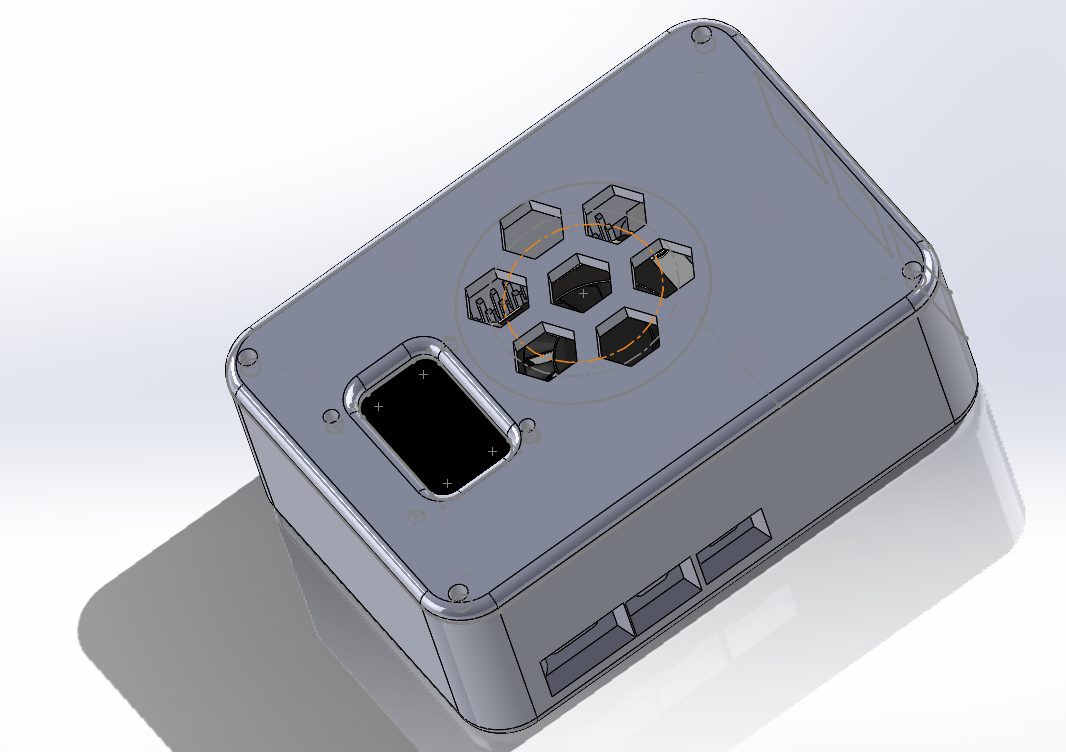
\includegraphics[width=0.85\textwidth]{figures/cad/case_full.png}
    \caption{Vista del conjunto completo de la carcasa de protección diseñada en
    SolidWorks 2022 para el prototipo. \textbf{Fuente:} Elaboración propia.}
    \label{fig:anexo-case-completo}
\end{figure}

\begin{figure}[H]
    \centering
    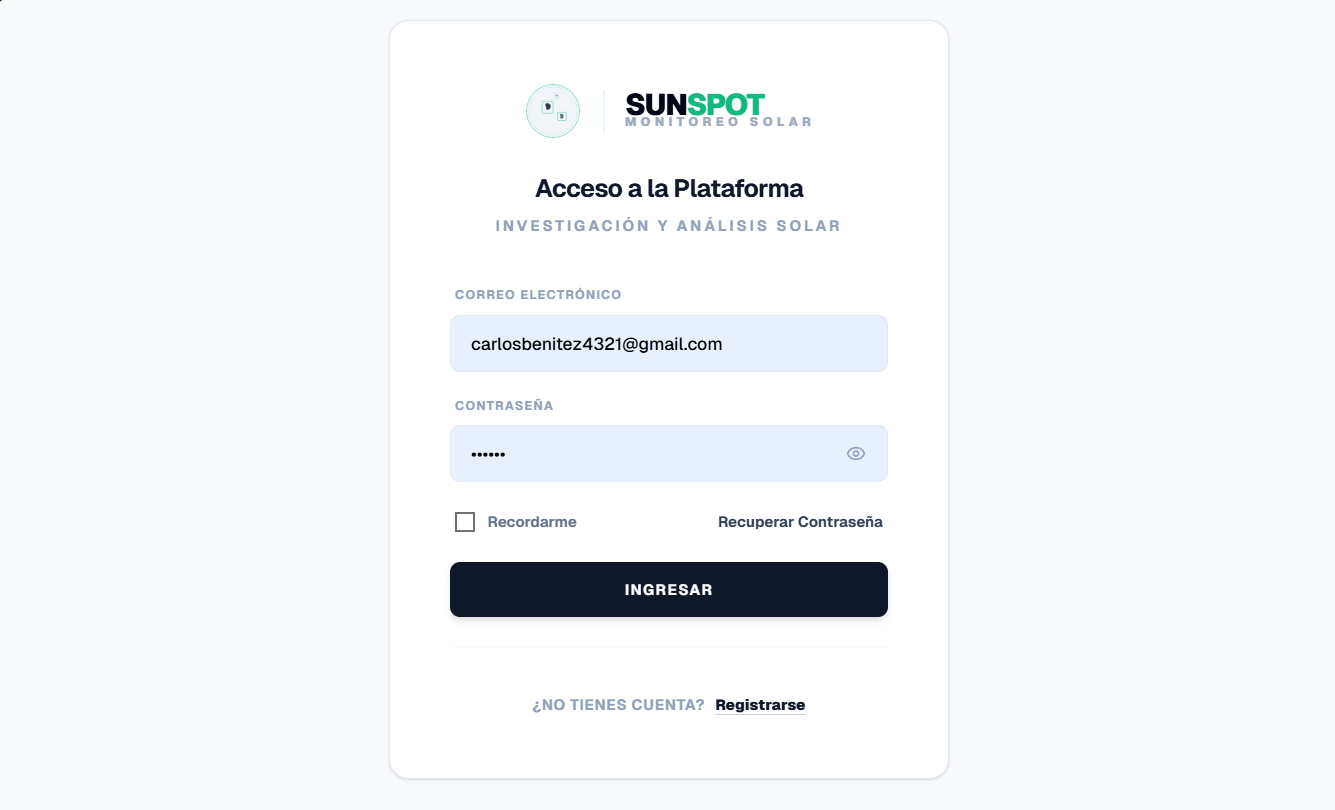
\includegraphics[width=0.95\textwidth]{figures/web/login.png}
    \caption{Pantalla de autenticación de la plataforma web utilizada para
    acceder al entorno de procesamiento y consulta. \textbf{Fuente:} Elaboración propia.}
    \label{fig:anexo-web-login-validacion}
\end{figure}

\begin{figure}[H]
    \centering
    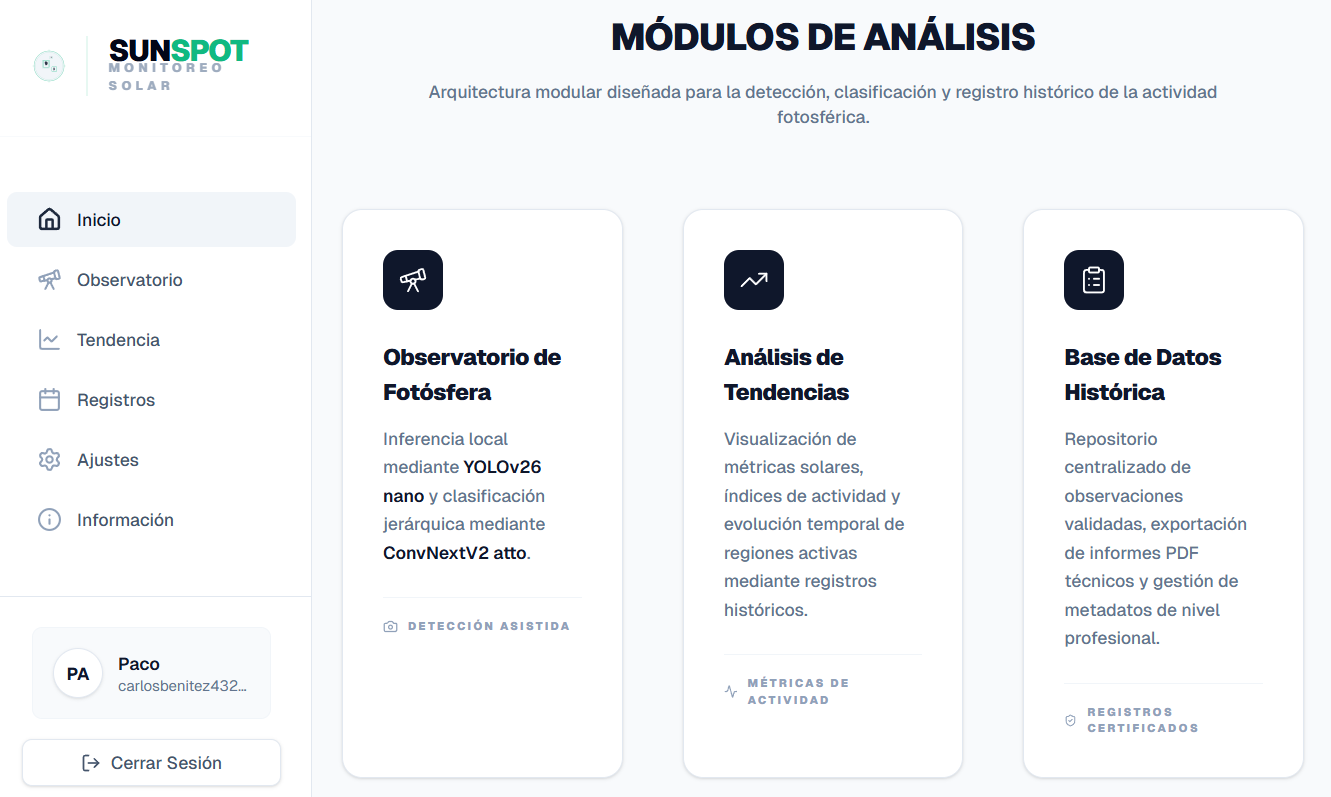
\includegraphics[width=0.95\textwidth]{figures/web/home.png}
    \caption{Vista principal de la plataforma web, desde la cual se organizan
    los módulos de procesamiento, consulta y visualización. \textbf{Fuente:} Elaboración propia.}
    \label{fig:anexo-web-home-validacion}
\end{figure}

\begin{figure}[H]
    \centering
    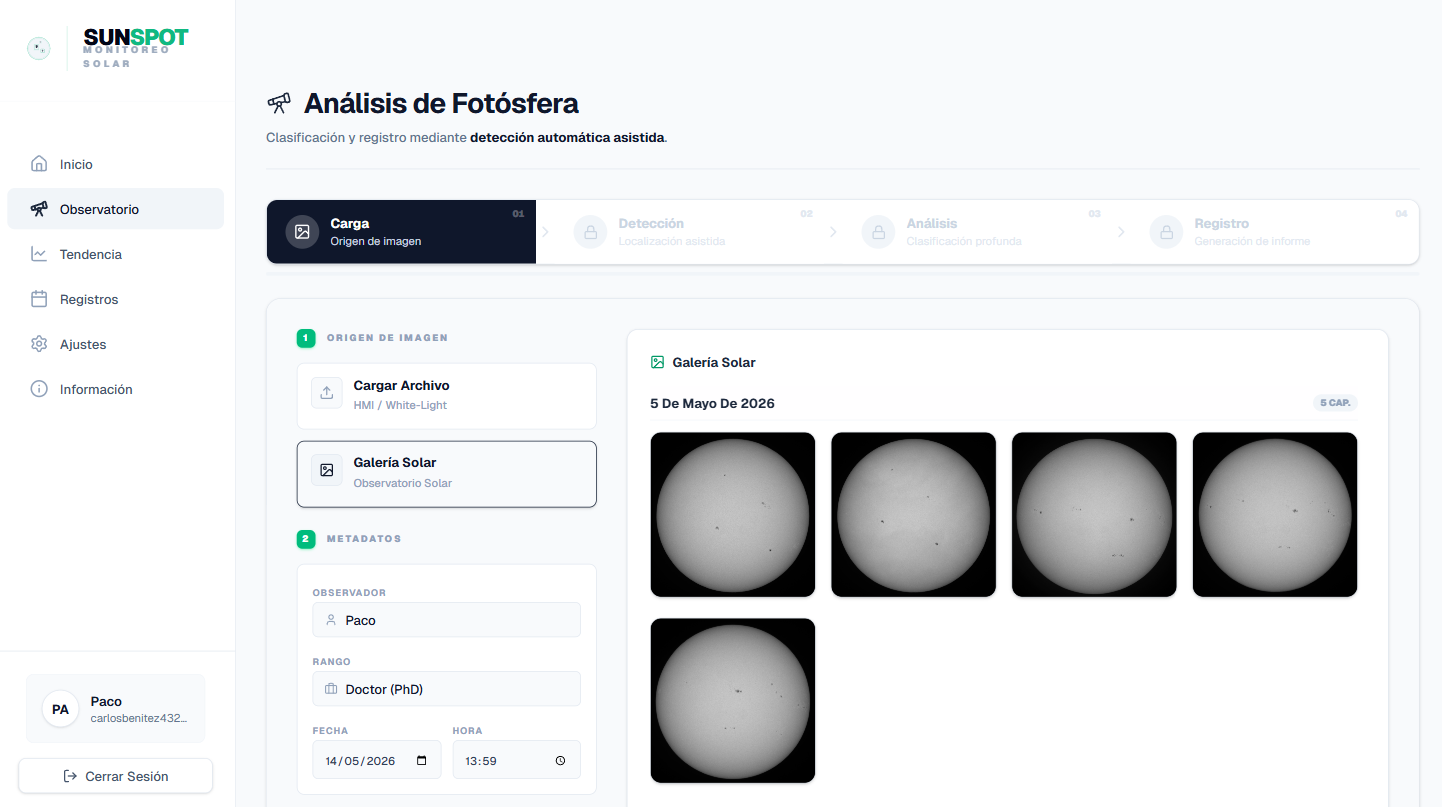
\includegraphics[width=0.95\textwidth]{figures/web/upload.png}
    \caption{Interfaz de carga de imágenes solares para iniciar el flujo de
    procesamiento dentro de la plataforma. \textbf{Fuente:} Elaboración propia.}
    \label{fig:anexo-web-carga-imagen-validacion}
\end{figure}

\end{appendices}